\chapter{Overview} \label{cap:overview}

\section{The Big Picture - the Overall Architecture [Herbert]}
\index{Architecture!Overview}
The following subsections are aiming on providing a rough overview on the
componentes of the Insieme project.

\subsection{The Compiler and the Runtime}
The Insieme project comprises two major components -- the \textit{Insieme
Compiler} and the \textit{Insieme Runtime}. The compiler's task is to convert
input codes based on various languages (C, C++, OpenCL) into a C-based
representation which, combined with the Runtime, can be compiled into a binary
exhibiting the behaviour as intended by the programmer of the input program.
During this process, the compiler is allowed to analyse, manipulate and
restructure the handled code (fragment) as long as the \textit{intended}
semantic of the program is not lost. Some of these transformations may include
look restructuring or reordering, optimization of message passing operations,
array manipulations, the introduction or elimination of parallel constructs or
the conversion of originally C based codes into OpenCL. 

The \textit{Runtime's} contribution on the other hand is to provide an abstract
interface to the underlying hardware infrastructure. It therefore requires the
handled program to follow a specific application model, allowing the runtime to
inspect and steer the execution of the corresponding code. The model, based on
work items, is covered within section \ref{sec:Overview.Runtime.AppModel}.
Further, the runtime offers interfaces for influencing the execution of parallel
codes (runtime-tuning) as well as for monitoring the execution of applications.
The latter allows to use collected data for post-mortem analyses as well as for
real-time decision making processes during the execution.

Although the Compiler is supporting other output formats too (e.g. plain
sequential C code), the ``native'' backend of the compiler is generating code
fitting the requirements of the runtime. Therefore the code is decomposed
into work-items and the required meta-information is collected via static code
analyses and stored within the corresponding \textit{implementation table}.

Form the Insieme developers point of view the Compiler and Runtime are
practically two different worlds. For once, the Compiler is implemented using
C++11 while the Runtime is based on C99. Furthermore, the Compiler constitutes a
library of passive functions to be orchestrated by the developer while the
runtime is a framework. Further general information regarding these two major
components will be covered within the following subsections. A detailed
coverage of the Compiler components can be found within chapter
\ref{cap:compiler} and for the Runtime within chapter \ref{cap:runtime}.


\subsection{The Compiler}

\subsubsection{The Goal}
The compiler provides a set of libraries including algorithms and data
structures to load, parse, analyses, manipulate and synthesize programs. Its
major goal is to provide these set of tools, enabling the research in
static program optimization. Furthermore, utilities supporting the
instrumentation, generation, compilation, (remote) execution and collection of
measurement results are supported \ref{sec:Driver.MeasureAndInstrument}. Hence,
the otherwise static part of the compiler can incorporate dynamic code
properties if desired.

A related requirement to the compiler is the desire of using the available
utilities as flexible as possible. Developers aiming on conducting compiler
research shell be enabled to easily combine the available means according to
their own requirements. To support this, all modules are required to deal with a
consistent data format used for representing the processed program code.
Consequently, a common internal representation for processed code is among the
most essential components of the compiler. In fact, it is forming the
centerpiece of the entire compiler infrastructure.

The Insieme parallel intermediate representation (INSPIRE or just IR if the
context is clear) is realizing this central component. This formal language has
been designed to express parallel concepts encountered within parallel
programming languages like OpenMP, OpenCL and MPI in a uniform way. The key idea
of the compiler is to convert all supported input languages into this unified,
streamlined IR. This way, for the compiler researcher focusing on improving
optimization in the context of parallel applications, this unified view provides
the benefit of already resolved ambiguities present within the input languages.
For researches being interested in a single input language this common internal
core ensures that similar utilities developed for related problems encountered
within other languages can be re-used. For instance, the extraction of a
parallel control flow graphs and algorithms operating on them
originally developed for analysing MPI codes can be reused for research on
OpenMP and OpenCL codes if required.\note{the pCFG has not yet been implemented}

Bottom-line -- the compiler is providing the means to represent parallel
programs as well as utilities to derive them from input codes, analyse and
manipulate them and finally modules converting the internal representation into
some form of processable output code (typically C). On top of this, a set of
utilities performing higher level functions like generic optimizations or
parameter studies are offered. All those are offered to provide an
infrastructure for compiler research on parallel codes.

\subsubsection{The Application Model}
As has been stated within the previous section, the internal application model
used to represent and process programs throughout the compiler is INSPIRE. It
represents applications based on an execution-oriented (in contrast to a
syntax-oriented) way. Hence, the actual execution should be modeled, not the
structure of the original code describing this execution. The IR offers basic
imperative structures including ordinary statements, conditions, switches,
for- and while-loops. However, functional concepts including higher-level
functions and lambdas are as well supported. Those features have especially been
included to support the recursive composition of arbitrary program constructs.
This should prevent the future need for extending the language. Every future
extensions should be supportable by combining existing constructs using
functional composition. The goal is to keep the language core as closed as
possible such that tools relying on those constructs need not be updated in case
new constructs are introduced over time.

Additionally, the IR has been designed to simplify analyses. The IR is kept
minimal and compact. Hence, only a small (yet not minimal due to concessions
toward intuitiveness) number of constructs are used to represent a program.
Details covering semantically irrelevant concepts like names of variables or
functions are as well discarded as the formatting of the input code. This way,
analyses can focus on the essential parts. The additional explicit
representation and unification of concepts like direct / indirect memory
accesses, memory management and parallelism (should) simplify the design and
implementation of code analyses. \note{at this stage, the development in this
direction hasn't reached a state to quantify the impact of the IR design on the
analyses with absolute certainty} Much more details on the Insieme IR can be
found within the INSPIRE language specification \cite{insieme_ir_spec}.


\subsubsection{Important Components}
\index{Architecture!Compiler Overview}
Figure \ref{fig:Overview.Compiler.Components} illustrates a basic overview on
the components involved within a typical compiler-based utility. 
\begin{figure}[tb]
	\centering
	%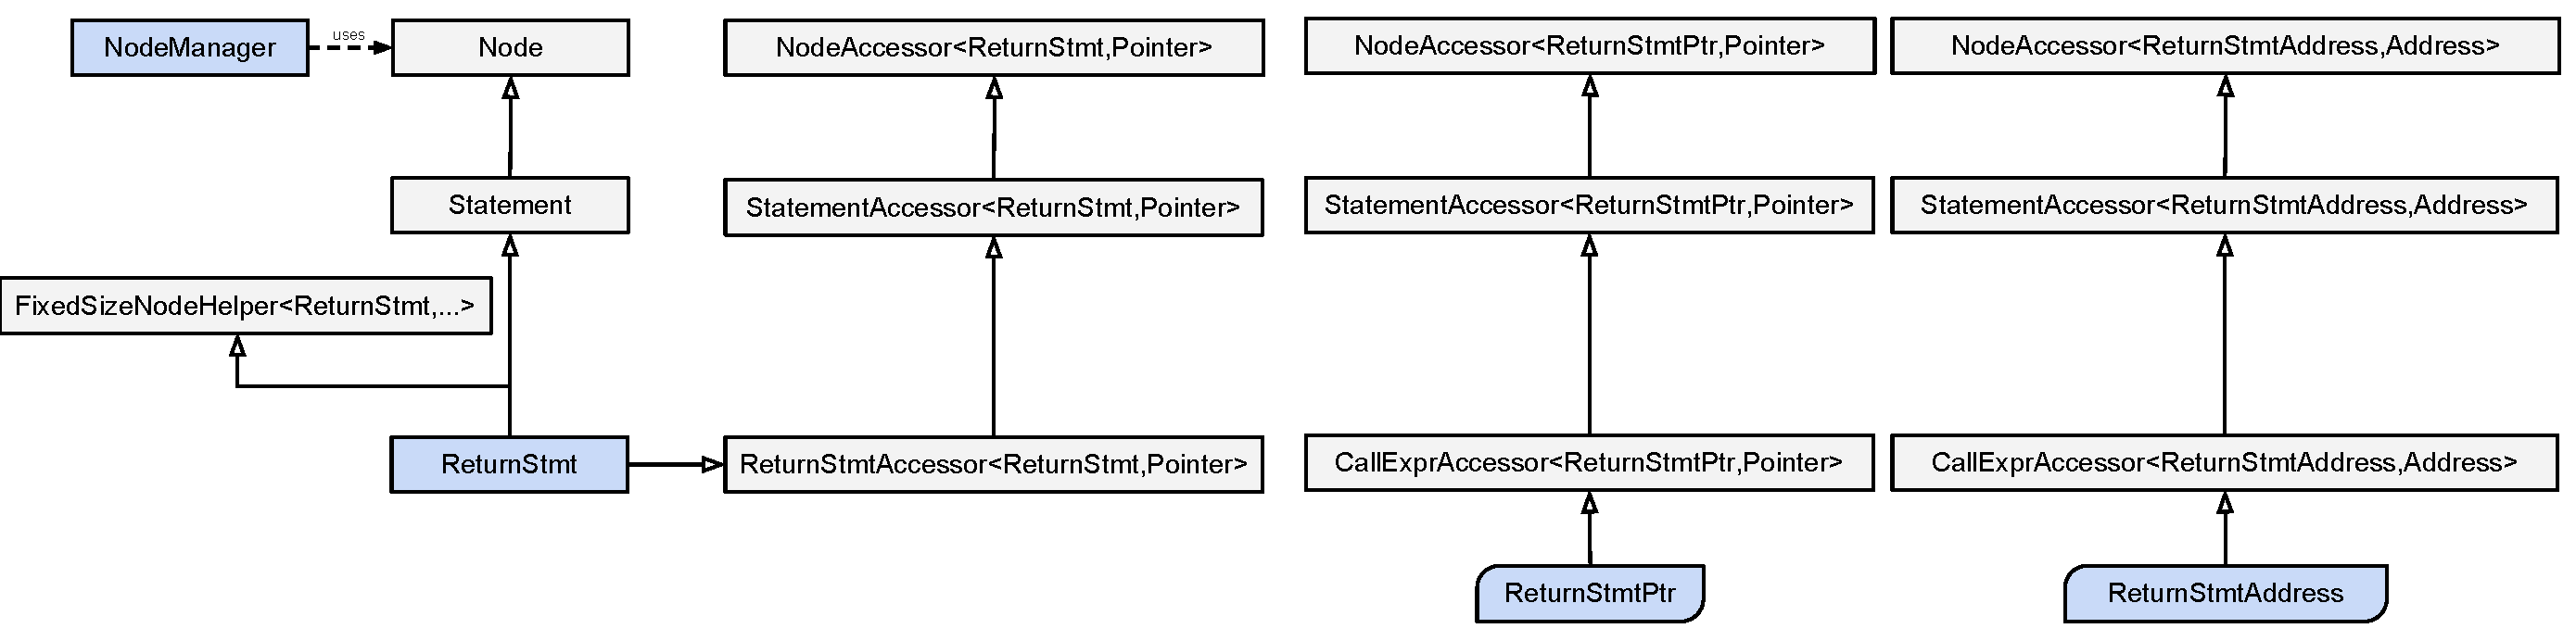
\includegraphics[width=\textwidth]{compiler/core/class_hierarchy_of_return_stmt.pdf}
	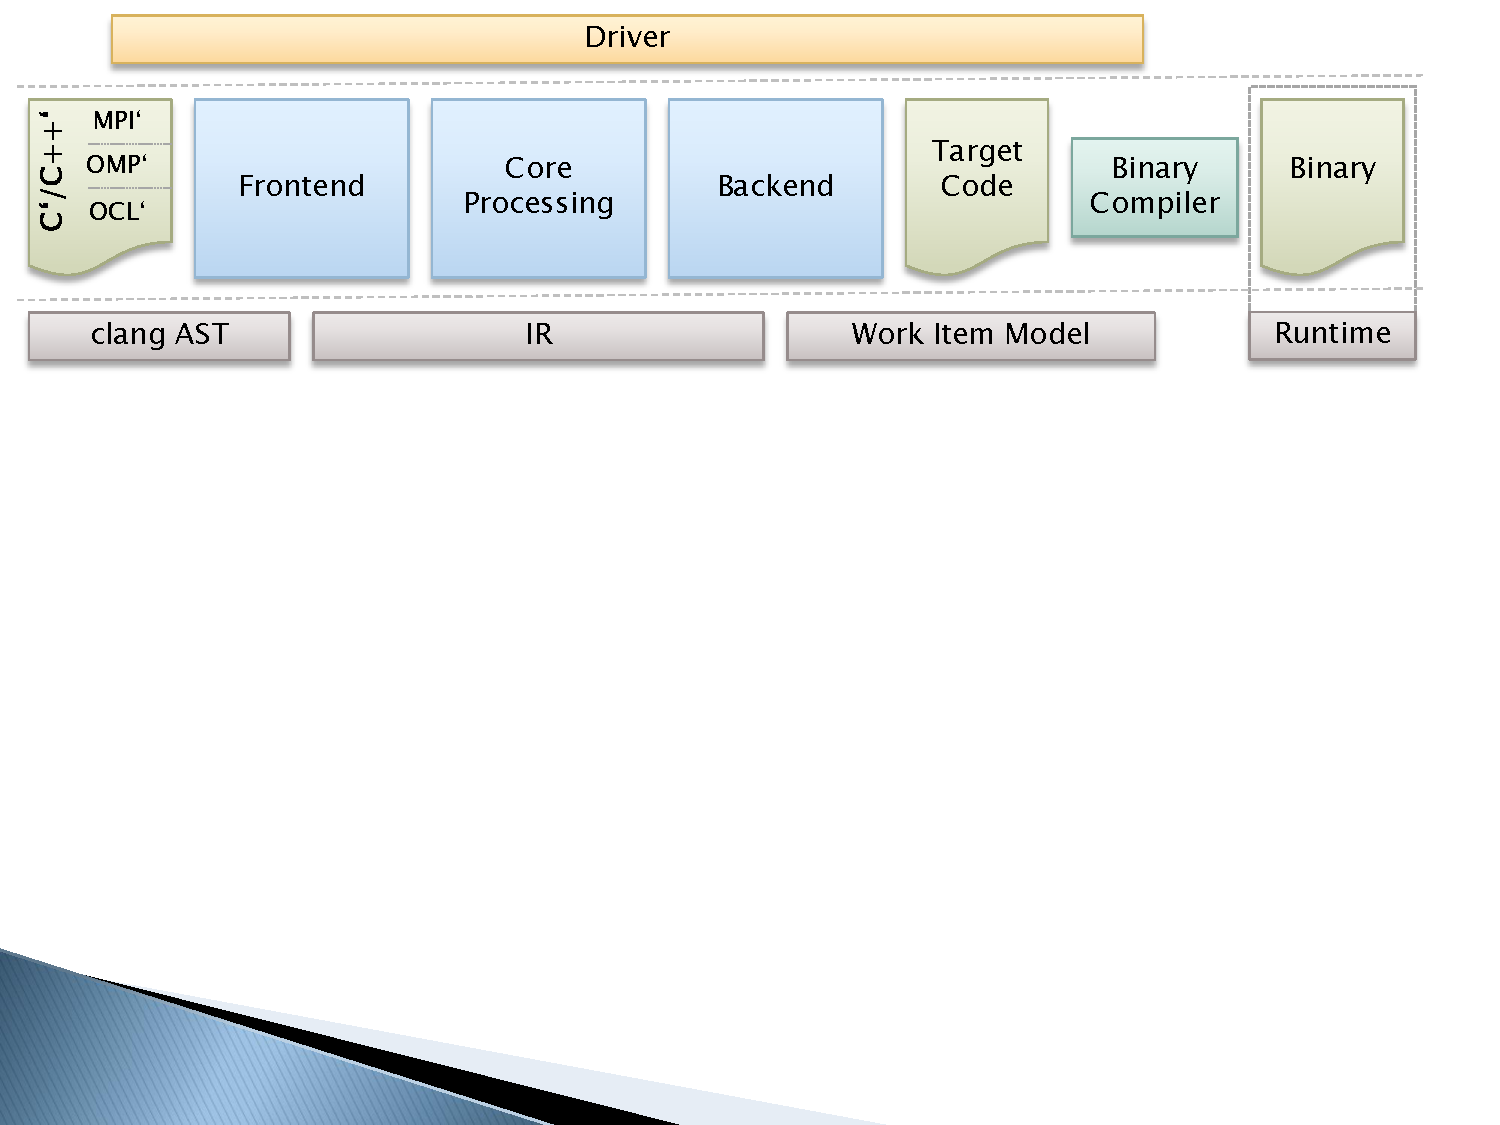
\includegraphics[width=\textwidth, trim=0 365 35 0, clip]{overview/architecture_overview.pdf}
	\caption{Overview on the Compiler's Components (blue) and the involved Program Representations (gray)}
	\label{fig:Overview.Compiler.Components}
\end{figure}
The green files represent the various formats client code is represented in
during its processing. It starts as a C/C++ code, potentially equipped using
MPI, OpenMP or OpenCL constructs. In general, no full coverage for all input
languages is guaranteed (hence the ' extending all the input languages). A
compiler frontend is used to convert this this code representation into the
internally used IR format. For more details on the frontend see section
\ref{sec:Insieme.Frontend}. Additional input languages may be supported.
Developers interested in this directions are welcome to contributed the
corresponding frontend implementation.

During the processing of the frontend the original source files are parsed and
converted into a clang AST (since the clang parser is used as a foundation for
the C/C++ frontend). The second phase of the frontend, the clang AST is
converted into the internal compiler IR (INSPIRE).

After the frontend the actual purpose of the implemented compiler utility can be
realized. At this point, the developer may chose to perform whatever analyses /
manipulation she thinks is suitable for realizing the intended objectives.
Chapter \ref{cap:compiler} provides an extensive overview on the offered
utilities. The one common element to all those operations is the format used for
describing program structures: INSPIRE. Every operation is accepting INSPIRE
code as an input and producing similar encoded codes as output.

Some compiler based utilities just aiming on static analyses of codes might
already stop here. However, in case code has been modified and shell be emitted,
a backend implementation has to be used. The basic role of the backend is to
convert the internal INSPIRE based code representation into a representation
which can be further processed by some external tool to ultimately obtain an
executable binary. As for the frontend, there are various backends
\footnote{There is a backend implemented by a bachelor thesis synthesizing Java
code}. While some may only be used to create sequential codes, the ``native''
backend is producing code exploiting the infrastructure offered by the Insieme
Runtime. Extensions for creating OpenCL kernel and host codes are as well
available. For more information, see section \ref{sec:Compiler.Backend}.

To utilize the Insieme Runtime, the internal IR based program representation has
to be converted into the work-item based application model required by the
runtime. This step is conducted within the backend. Furthermore, constructs
emitting lambdas and clousures are encoded into equivalent C constructs. The
result target code is based on C, satisfying the requirement specified by the
runtimes application model.

The generated target code finally has to be compiled together with the
headers of the Runtime libraries using some third party compiler (e.g. GCC) to
obtain a binary which finally can be executed on any target architecture
supporting the Insieme Runtime infrastructure.

On top of all those steps a Compiler Driver is located. It is implementing the
main procedure, hence the entry point of the application and it is orchestrating
all the remaining components. It is responsible for selecting the input files
(typically based on some input parameters), invoking the various parsing,
processing and synthesizing steps in some case even triggering the third-party
binary compiler to produce an executable result. Although many utilities
supporting the implementation of the various steps are available (e.g. command
line parameter parsing or the invocation of a third-party binary compiler) the
implementation of the actual driver is left to the compiler researcher for a
maximum of flexibility. 

For conducting integration tests and basic experiments, one main executable is
included within the project. However, it should not be (further)
customized/extended to serve additional purposes. In general, to keep the
implementation manageable, developers are encouraged to build specialized
executables for their specific requirements within an isolated scope.



\subsubsection{Implementation Details}
From the developers point of view, the compiler is a large library of utilities.
Although there is a main executable assembling a basic pipeline of steps for
loading, processing and synthesizing codes using a flexible selection of front
and backends, in general users are encouraged to create individual executables
for their tasks. To keep executables structured, the \textit{playground} module
has been set up within the source repository. This module can be used as a
foundation for building new executables covering any required workflow. The
build environment is automatically generating build-targets for executables for
any file using the \file{cxx} extension (see \ref{sec:Infrastructure.Build}).

As a consequence of this design decision, any component / module within the
compiler has to follow the library concept by implementing some passive module
being triggered by an external control flow. To simplify the composition of
various utilities, each module should aim for providing clean interfaces for end
users. Hence, if possible, a single header file should be used. Also, all
parameters effecting the process shell be configurable at a single position,
ideally using locally allocated data structures to allow the (simple)
integration of multiple instances of the same module within a single process
instance.


\subsection{The Runtime}

\subsubsection{The Goal}
The major goal of the runtime is to provide an abstract machine interface
to applications. It thereby does not effect the standard instruction set
supported by the underlying architecture. The abstraction is limited to some
higher-level concepts, im particular including threads, parallel loops,
synchronization and communication mechanisms. These constructs form the
foundation for any parallel application. The optimizer within the runtime 
aims on improving the performance of the executed program code by coordinating
and tuning the utilization of those means and the associated resources.

In addition to the parallelization and communication primitives the runtime also offers support for the integration of generic tuning capabilities, so-called \textit{tunable knobs} \index{Tunable Knobs} \note{Knobs have not yet
been implemented}. This kind of optimization utility can be included within the
executed application code at performance relevant locations, allowing the
runtime optimizer to influence the execution of the code. For instance, the
value of a knob may determine the tiling factors of a loop, the cut-off of a
recursive procedure or switch between various algorithms solving the same
problem. The runtime offers support for tuning those knobs. \note {not yet
:)}

Another set of functionality offered by the runtime are monitoring utilities.
The runtime offers an API for tracking resource requirements and the status of
hardware counters during the execution of code. The collected information may be
used for post-mortem program analyses or already during the execution for future
decision making processes \note{full API not yet implemented}.

\note{Update this section when the distributed runtime has been realized} There
are plans to extend the runtime to be extended to a distributed runtime, hence
abstracting away the fact that the actual underlying architecture is a
distributed memory system. Unlike existing approaches, this idea would not
``simply'' simulate one virtual, large, shared address space and run the
application on top of it. Instead it would exploit the extra information
regarding the program structure provided by any application satisfying the
runtime's application model to distribute codes effectively. However, these
plans haven't yet be realized.


\subsubsection{The Application Model} \label{sec:Overview.Runtime.AppModel}
The runtime requires any application to be processed using its infrastructe to
obey a predefined interface -- frequently refered to as the work-item or the
runtime model. In particular, all codes to be executed using the runtime have to
be organized within \textit{work items}. \index{Work Items} Essentially, a work
item is a piece of code that can be invoked by providing the required input data
-- similar to procedures. However, work-items have a fixed signature, hence all
of them can be generically invoked by the runtime. Further, for each work-item,
meta-information regarding the accepted input parameters is offered within a
so-called \textit{implementation table}. Furthermore, unlike ordinary
procedures, the work-load of a single invocation may be distributed among
multiple threads. The exact number can be determined by the runtime. The work-item implementation will use those threads to conduct its task efficiently. Last but not least, each work-item can offer multiple implementations -- each specialized for particular scenarios -- to the runtime. One implementation may be chosen for a serial execution, not including any synchronization primitives. Another may be used for conducting the computation on an accelerator. The characteristic of the offered implementations is described by additional meta-information offered within the \textit{implementation table}.

In addition to the work-items, data is also organized within data-items.
\note{data items are not yet implemented} Applications running within the
runtime are not supposed to manage their own heap memory (although technically
they are not prohibited from doing so), they are requested to let the runtime
manage the corresponding operations. Every data-item has a type, a dimension
(0,1,2,\ldots dimensional array) and a size (number of elements along each
dimension). Further, data items may be stored in a distributed fashion. Hence,
the runtime is not guaranteeing that arrays are actually stored in a consecutive
order within memory. Whenever a work-item requires access to a data-item it has
to state a request within its associated requirement function. Within this
request a sub-range of the full data-item and an access mode (read only, write
only, write first, \ldots) can be stated. The runtime's obligation is to
organize a valid instances of the requested memory portion. In a simple system,
those operations might just forward pointers to the unique copy managed
somewhere within the memory. However, in a NUMA system (or potentially even
within a distributed memory system) this additional knowledge on the data
requirements of the work-items can be exploited for improving data locality. For
instance, read only memory blocks may be duplicated several times throughout
the system to speed up memory accesses. 

All this meta-information regarding the application should offer research
on runtime based decision making processes a large potential for optimization
and tuning opportunities. More details regarding the application model and the
runtimes internal organization can be found within chapter \ref{cap:runtime} and
the Runtime Specification \cite{insieme_runtime_spec}.

\subsubsection{Runtime Modes}
The Runtime has been designed ot operate within two operation modes. In both
cases the same application can be used:

\begin{itemize}
  \item \textbf{Standalone Runtime} \index{Runtime Modes!Standalone}this mode is
  intended for handling a single application. In this version, the Insieme
  Runtime is ``merged'' into its managed application. The \srcCodeInl{main} of
  the handled program has to be replaced by a short routine conducting the
  initialization of the runtime and starting up a standalone-runtime procedure.
  This procedure is setting up the required infrastructure (workers, \ldots) and
  invoking the original \srcCodeInl{main}. As soon as the control flow of the
  original \srcCodeInl{main} terminates, the Runtime is shut down gracefully.
   
  \item \textbf{Runtime as a Service}\index{Runtime Modes!Runtime as a Service}
  in this second runtime mode, the Runtime is continuously executed on a server
  machine and managing the available resources. Client codes, implemented
  according to the application model may be submitted to this Runtime Service
  (by submitting a reference to a compiled dynamic library including the actual
  client code) for execution. The runtime will load the library, invoke the
  mandatory initialization function and trigger the computation of a
  user-specified entry point. Unlike the stand-alone version, this variant may
  coordinate the resource usage of multiple client codes on a shared hardware
  platform simultaneously.
\end{itemize} 

\subsubsection{Important Components [Peter]} \label{sec:overview:runtime:components}
Figure \ref{fig:Overview.Runtime.Components} illustrates a basic overview on
the components comprising the Insieme runtime system. \index{Runtime!Components Overview}
\begin{figure}[tb]
	\centering
	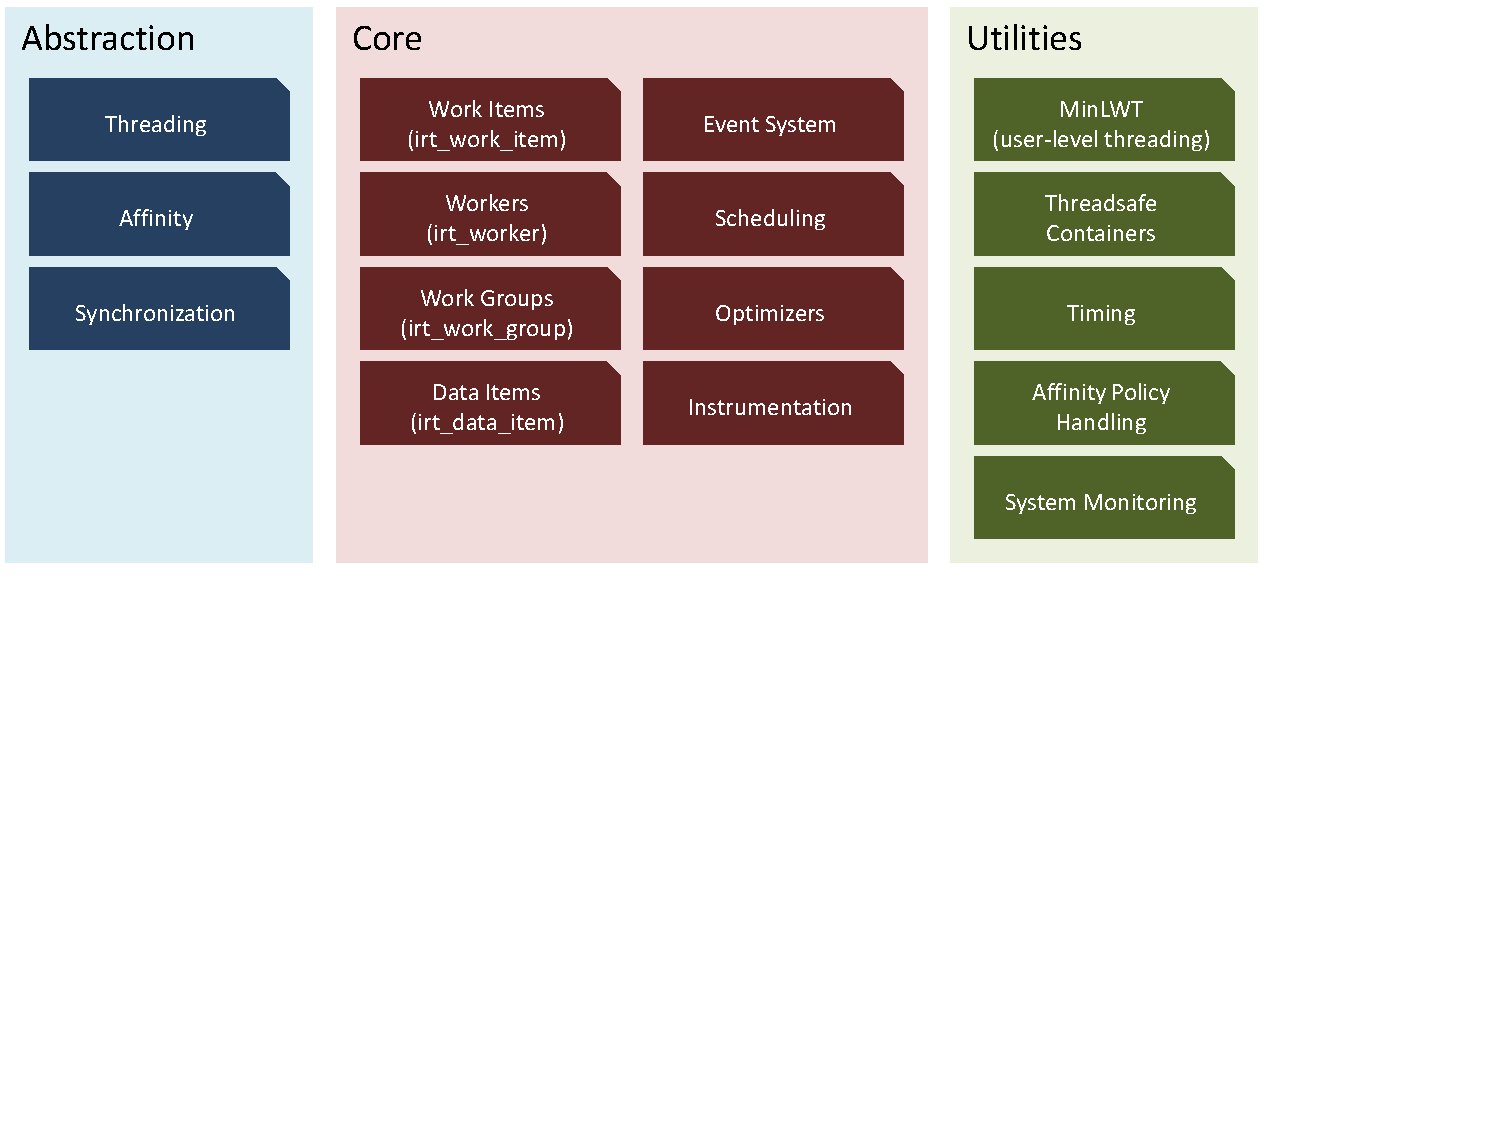
\includegraphics[width=\textwidth, trim=0 9cm 4cm 0,
	clip]{pics/runtime/overview_components.pdf}
	\caption{Overview on the Runtime's components}
	\label{fig:Overview.Runtime.Components}
\end{figure}

The components are grouped in three major categories:
\begin{description}
  \item[Abstraction] Components that abstract facilities provided from the OS level to enable portability.
  \item[Core] Components providing the core functionality of the runtime system.
  \item[Utilities] Modules which offer functionality required by, but independent from the runtime core.
\end{description}

The \textbf{abstraction} layer is currently still under construction. \note{update when progress is made on the abstraction layer} It is intended to encapsulate basic OS-level threading, synchronisation, and other system-specific tasks (e.g. affinity settings) and provide implementations for each supported platform.

\textbf{Utilities} are components that are largely independent of the rest of the runtime, but are used by it to accomplish its tasks. Currently, the following utilities are implemented.
\begin{description}
\item[MinLWT] A user-level (lightweight) threading library. Provides high-performance implementations for some architecutures, with a thread switching overhead of less than 10 cycles. A fallback implementation using the POSIX \texttt{ucontext} library is also provided for unsupported hardware.
\item[Threadsafe Containers] High-performance, threadsafe container structures based on atomic operations and fine-grained locking. Includes deques, counting deques and lookup tables.
\item[Timing] Highly accurate timers and sleeping functions, as well as calibration support to convert to/from CPU ticks and time units.
\item[Affinity Policy Handling] Generates affinity masks from policies and converts between internal Insieme and OS-level thread numbering.
\item[System Monitoring] Provides information about the system state, such as the current externally generated CPU load.
\end{description}

Finally, \textbf{core} components encompass the central implementation of the runtime. 
\begin{description}
\item[Work Items] The basic unit of work in the runtime system. A user-level thread with additional meta-information about its data requirements and properties, with any number of implementations.
\item[Workers] OS-level threads that accomplish the scheduling and management of work items.
\item[Work Groups] Groups of work items which can perform aggregated operations. Barriers, work distribution methods and aggregated data exchange functions operate on work groups.
\item[Data Items]\note{Not fully implemented} The basic unit of data in the runtime. Programs use data items to enable the runtime to optimize the distribution and usage of data throughout a program.
\item[Event System] A generic system that allows the components of the runtime -- work items, workers, groups and data items -- to generate and recieve events. Events consist of a source, which is one of the above objects, an event ID and an event lambda, which is a combination of data and function executed when the event occurs.
\item[Scheduling] This component includes two currently separated systems: task scheduling and loop scheduling. Task scheduling implements the distribution of work items to workers, by means such as task stealing. Loop scheduling distributes the iterations of a loop among the members of a work group.
\item[Optimizers] The optimization of various processes performed by components listed above, such as scheduling and data distribution, is relegated to the optimizers in this module.
\item[Instrumentation] Instrumentation provides meta-information about the programs executed by the runtime as well as the runtime itself, either during execution or post-mortem.
\end{description}

A more detailed examintation of each of these components is provided in chapter \ref{cap:runtime}.


\subsubsection{Implementation Details [Peter]}
Unlike the compiler which is essentially a large library, the Runtime is
designed as a framework from the runtime developers' point of view. Hence, within the runtime the control flow is determined by the core system as well as the executed program code and can not be (significantly) changed. Runtime developers can merely effect decision making processes within this pre-determined fixed infrastructure -- which should be sufficient for most ventures. However, in case the pre-determined ``points of influence'' are insufficient, modifications of the framework may need to be conducted.

A particular focus within the runtime lies on program \textit{efficiency} and
\textit{performance}. Since every operation executed within the runtime adds up
to the instructions processed for running client code and therefore
(potentially) to its execution time, all implementations have to be as efficent
as possible. This has an impact on how interfaces should be designed. The basic interface and calling conventions of functions should focus on performance, additional interfaces which simplify usability can subsequently be added on top of these base interface if required.

Furthermore, since the Runtime is implemented in C which does not support name
spaces, more constraints have to be enforced regarding the coding standards than
within the compiler to avoid a babylonian confusion caused by a large number of
different conventions.

\section{The Insieme Coding Philosophy}

\begin{comment}
\begin{itemize}
  \item Insieme Compiler vs. Insieme Runtime
  \item Compiler - tool kit to build compiler related utilities,
  transformations, analysis, \ldots
  \item Runtime - framework controlling the execution of an application;
  extended by providing alternative implementations of given functionality; flow
  of control is dictated by the runtime
  \item Point out difference: Compiler = Library = Toolkit, Runtime = Framework
\end{itemize}


State that:
\begin{itemize}
  \item Each ``component'' should represent a closed entity - usable via a simple
  user friendly interface without the requirement of modifying internal code
  \item Each component has to declare itself as a ``framework'' or ``library'' -
  define those two terms!
  \item Extendable by design - not re-design
  \item Coding standards
\end{itemize}
\end{comment}